% !TEX root = ../Report.tex
% ======================================================================
\chapter{Implementation}
\label{ch:implementation}
% ======================================================================

This chapter documents how the design was realised in code, covering major
implementation modules and the reasoning behind key decisions.

\section{Backend Structure}
The backend is a Node.js and Express application \cite{ref_node_about,ref_express}.
The main server file configures:
\begin{itemize}
  \item EJS templating for UI routes,
  \item JSON body limits for planner payloads,
  \item authentication sessions (\texttt{gitrip\_sid}),
  \item security headers and rate limiting,
  \item caching for external API calls (geocoding and weather).
\end{itemize}

\subsection{Database Layer}
The database layer uses \texttt{better-sqlite3} and maintains schema migrations
in a single module. Commit rows store JSON fields (\texttt{parents},
\texttt{snapshot}) as strings and are deserialised on load. The schema
intentionally does not enforce foreign keys at the SQLite level; relationships
are handled logically by the application. Indexes are created on all
foreign-key columns (e.g., \texttt{commits.repo\_id},
\texttt{branches.repo\_id}, \texttt{repo\_stars.repo\_id/user\_id}) to
maintain query performance as the number of repositories and commits grows.

\subsection{Error Handling}
All error responses sent to users use generic messages (e.g., ``Planner error.
Please try again.'') rather than exposing internal error details. Full error
information is logged server-side via \texttt{console.error} for debugging.
This prevents information leakage of internal paths, stack traces, or
dependency details that could aid reconnaissance.

\section{Planner Implementation}
\label{sec:planner-impl}
The auto-scheduler is implemented in \texttt{server/planner.js}. Key components
include:
\begin{itemize}
  \item \textbf{Time helpers:} \texttt{toMin} and \texttt{toHHMM}.
  \item \textbf{Matrix building:} ORS matrix for non-transit; null for transit.
  \item \textbf{Ordering logic:} strict order handling (absolute or relative);
        when no strict orders exist, Held-Karp exact solver for $N \leq 12$
        \cite{ref_tsp_study}, otherwise Nearest Neighbour with 2-Opt refinement
        \cite{ref_nn_tsp,ref_nn_2opt_hybrid}.
  \item \textbf{Constraint fit check:} \texttt{applyOpeningHours} integrates
        active hours, desired windows, fixed-time behaviour, and opening-hours
        nudging.
  \item \textbf{Packing loop:} schedules preferred-day buckets first, then
        unassigned stops, spilling to later days or overflow when necessary.
\end{itemize}

The planner records travel minutes (\texttt{prevTravelMin}) and effective route
mode per leg, including detection of transit vs walking in cases where the
transit provider returns walking-only legs.

The ordering stage uses three strategies depending on instance size, presented in Algorithms~\ref{alg:nn}--\ref{alg:heldkarp}. The NN heuristic (Algorithm~\ref{alg:nn}) greedily selects the closest unvisited stop; if no finite edge exists from the current node, remaining stops are appended in their original input order. The 2-Opt refinement (Algorithm~\ref{alg:twoopt}) iteratively reverses sub-segments to reduce total cost, keeping the origin fixed and running up to 4 sweeps or until no improvement is found. The Held-Karp solver (Algorithm~\ref{alg:heldkarp}) solves for the shortest \emph{path} (open tour), not a cycle, unlike the classic TSP formulation.

\begin{algorithm}[H]
  \caption{Nearest Neighbour heuristic - greedy $O(N^2)$ path construction.}
  \label{alg:nn}
  \begin{algorithmic}[1]
    \Require travel-time matrix $M$, start index $s$
    \Ensure  visit order $\mathit{order}$
    \State $\mathit{order} \gets [s]$; \; $\mathit{used}[s] \gets \textbf{true}$
    \While{$|\mathit{order}| < N$}
      \State $\mathit{cur} \gets \mathit{order}.\mathrm{last}$
      \State $\mathit{best} \gets \arg\min_{j \notin \mathit{used}} M[\mathit{cur}][j]$
      \If{$\mathit{best}$ exists}
        \State $\mathit{used}[\mathit{best}] \gets \textbf{true}$; \;
               append $\mathit{best}$ to $\mathit{order}$
      \Else
        \State append all remaining unvisited nodes in original index order
        \State \textbf{break}
      \EndIf
    \EndWhile
    \State \Return $\mathit{order}$
  \end{algorithmic}
\end{algorithm}

\begin{algorithm}[H]
  \caption{2-Opt local search refinement.}
  \label{alg:twoopt}
  \begin{algorithmic}[1]
    \Require visit order $\mathit{order}$, travel-time matrix $M$
    \Ensure  improved visit order $\mathit{best}$
    \State $\mathit{best} \gets \mathit{order}$; \;
           $\mathit{bestCost} \gets \Call{PathCost}{\mathit{best}, M}$
    \For{$\mathit{pass} \gets 1$ \textbf{to} $4$}
      \State $\mathit{improved} \gets \textbf{false}$
      \For{$i \gets 1$ \textbf{to} $N - 3$}
        \Comment{skip index 0 to fix origin}
        \For{$k \gets i + 1$ \textbf{to} $N - 2$}
          \State $\mathit{cand} \gets \mathit{best}$ with segment $[i \ldots k]$ reversed
          \If{$\Call{PathCost}{\mathit{cand}, M} < \mathit{bestCost}$}
            \State $\mathit{best} \gets \mathit{cand}$; \;
                   $\mathit{bestCost} \gets \Call{PathCost}{\mathit{cand}, M}$; \;
                   $\mathit{improved} \gets \textbf{true}$
          \EndIf
        \EndFor
      \EndFor
      \If{$\lnot\mathit{improved}$} \textbf{break} \EndIf
    \EndFor
    \State \Return $\mathit{best}$
  \end{algorithmic}
\end{algorithm}

\begin{algorithm}[H]
  \caption{Held-Karp exact solver - bitmask DP in $O(2^N \cdot N^2)$, used for $N \leq 12$.}
  \label{alg:heldkarp}
  \begin{algorithmic}[1]
    \Require travel-time matrix $M$, start index $s$
    \Ensure  optimal visit order $\mathit{order}$, cost
    \State $N \gets |M|$; \; $\mathit{FULL} \gets 2^N - 1$
    \State $\mathit{dp}[\mathit{mask}][j] \gets \infty$ for all $(\mathit{mask}, j)$
    \State $\mathit{parent}[\mathit{mask}][j] \gets -1$ for all $(\mathit{mask}, j)$
    \State $\mathit{dp}[2^s][s] \gets 0$
      \Comment{base case: start at $s$}

    \Statex
    \For{$\mathit{mask} \gets 0$ \textbf{to} $\mathit{FULL}$}
      \If{bit $s$ not set in $\mathit{mask}$} \textbf{continue} \EndIf
      \For{$j \gets 0$ \textbf{to} $N-1$ where bit $j$ set in $\mathit{mask}$}
        \For{$k \gets 0$ \textbf{to} $N-1$ where bit $k$ \emph{not} set in $\mathit{mask}$}
          \State $\mathit{nm} \gets \mathit{mask} \;\mathbin{|}\; 2^k$
          \If{$\mathit{dp}[\mathit{mask}][j] + M[j][k] < \mathit{dp}[\mathit{nm}][k]$}
            \State $\mathit{dp}[\mathit{nm}][k] \gets \mathit{dp}[\mathit{mask}][j] + M[j][k]$
            \State $\mathit{parent}[\mathit{nm}][k] \gets j$
          \EndIf
        \EndFor
      \EndFor
    \EndFor

    \Statex \Comment{--- Reconstruct optimal path ---}
    \State $\mathit{bestEnd} \gets \arg\min_j \mathit{dp}[\mathit{FULL}][j]$
    \State $\mathit{order} \gets []$; \; $\mathit{mask} \gets \mathit{FULL}$; \;
           $\mathit{cur} \gets \mathit{bestEnd}$
    \While{$\mathit{cur} \neq -1$}
      \State prepend $\mathit{cur}$ to $\mathit{order}$
      \State $\mathit{prev} \gets \mathit{parent}[\mathit{mask}][\mathit{cur}]$; \;
             clear bit $\mathit{cur}$ from $\mathit{mask}$; \;
             $\mathit{cur} \gets \mathit{prev}$
    \EndWhile
    \State \Return $(\mathit{order},\;\mathit{dp}[\mathit{FULL}][\mathit{bestEnd}])$
  \end{algorithmic}
\end{algorithm}

Figure~\ref{fig:planner_flow} shows the auto-scheduler flowchart. The algorithm builds an ORS travel-time matrix (with Haversine fallback), orders stops (strict constraints, Held-Karp for $N \leq 12$, or NN and 2-Opt), then partitions them into preferred-day buckets and an unassigned pool. Phase~1 schedules preferred-day stops on their assigned day, sending unfitting stops directly to overflow. Phase~2 schedules unassigned stops greedily, spilling to subsequent days (retrying the same stop) or overflow when no days remain. The cursor is initialised with a focus-dependent shift (morning, midday, or afternoon).

\begin{figure}[H]
  \centering
  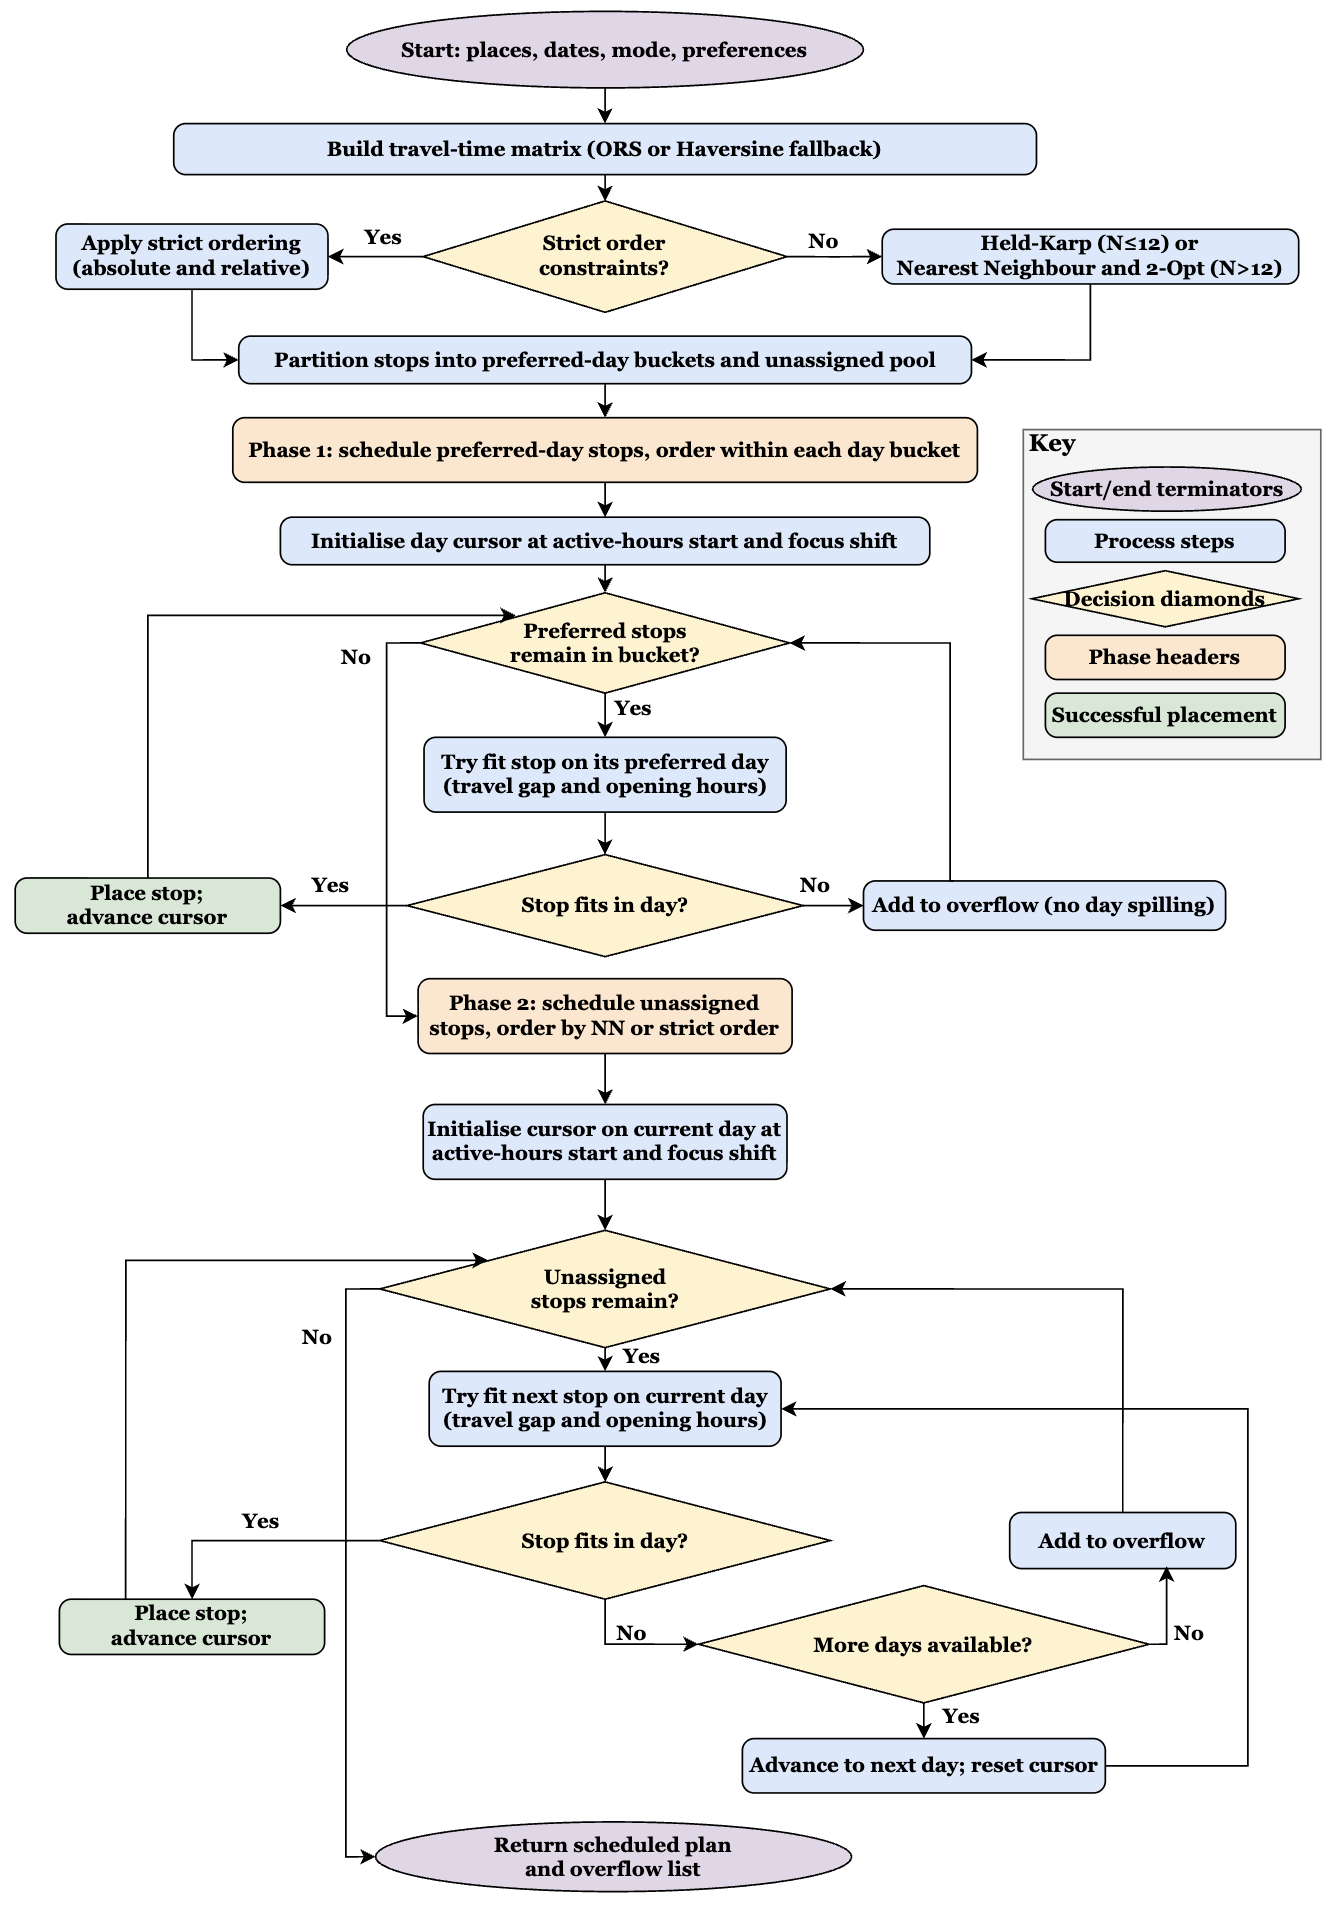
\includegraphics[width=0.9\textwidth]{Chapter6/auto-scheduler-flowchart.png}
  \caption{Auto-scheduler flowchart.}
  \label{fig:planner_flow}
\end{figure}

\begin{algorithm}[H]
  \caption{Auto-scheduler pseudocode (simplified from \texttt{server/planner.js}, 783~lines).}
  \label{alg:planner}
  \begin{algorithmic}[1]
    \Require $\mathit{places}$, $\mathit{days}$, $\mathit{activeStart}$, $\mathit{activeEnd}$, $\mathit{focus}$, $\mathit{transport}$
    \Ensure  $\mathit{days}$ (each with scheduled stops), $\mathit{overflow}$

    \Statex \Comment{--- Initialisation ---}
    \State $M \gets \Call{BuildTravelMatrix}{\mathit{places},\;\mathit{transport}}$
      \Comment{ORS or Haversine fallback}
    \If{$|\mathit{places}| \leq 12$}
      \State $\mathit{ordered} \gets \Call{HeldKarp}{\mathit{places},\;M}$
        \Comment{exact optimal order}
    \Else
      \State $\mathit{nnOrder} \gets \Call{NearestNeighbour}{\mathit{places},\;M}$
      \State $\mathit{ordered} \gets \Call{TwoOpt}{\mathit{nnOrder},\;M}$
    \EndIf
    \State partition $\mathit{ordered}$ into $\mathit{assignedByDay}$ and $\mathit{unassigned}$
    \State $\mathit{focusShift} \gets$ offset from $\mathit{focus}$
      \Comment{0, $\lfloor\mathit{span}/3\rfloor$, or $\lfloor\mathit{span}/1.8\rfloor$}

    \Statex
    \Statex \Comment{--- Phase 1: preferred-day stops ---}
    \For{each $\mathit{day}$ in $\mathit{days}$}
      \State $\mathit{cursor} \gets \mathit{activeStart} + \mathit{focusShift}$
      \For{each $\mathit{stop}$ in $\mathit{assignedByDay}[\mathit{day}]$}
        \State $\mathit{travel} \gets M[\mathit{last},\;\mathit{stop}]$
        \State $\mathit{propose} \gets \mathit{cursor} + \mathit{travel}$
        \State $(a, b, \mathit{fits}) \gets \Call{ApplyOpeningHours}{\mathit{stop},\;\mathit{propose},\;\mathit{activeEnd}}$
        \If{$\mathit{fits}$}
          \State schedule $\mathit{stop}$ at $[a, b]$; \; $\mathit{cursor} \gets b$
        \Else
          \State append $\mathit{stop}$ to $\mathit{overflow}$
        \EndIf
      \EndFor
    \EndFor

    \Statex
    \Statex \Comment{--- Phase 2: unassigned stops (greedy with spill) ---}
    \State $d \gets 0$; \; $\mathit{cursor} \gets \mathit{activeStart} + \mathit{focusShift}$
    \For{each $\mathit{stop}$ in $\mathit{unassigned}$}
      \State $\mathit{travel} \gets M[\mathit{last},\;\mathit{stop}]$
      \State $\mathit{propose} \gets \mathit{cursor} + \mathit{travel}$
      \State $(a, b, \mathit{fits}) \gets \Call{ApplyOpeningHours}{\mathit{stop},\;\mathit{propose},\;\mathit{activeEnd}}$
      \If{$\mathit{fits}$}
        \State schedule $\mathit{stop}$ on day $d$ at $[a, b]$; \; $\mathit{cursor} \gets b$
      \Else
        \While{$\lnot\mathit{fits}$ \textbf{and} $d < |\mathit{days}|$}
          \State $d \gets d + 1$; \; $\mathit{cursor} \gets \mathit{activeStart} + \mathit{focusShift}$
          \State $(a, b, \mathit{fits}) \gets \Call{ApplyOpeningHours}{\mathit{stop},\;\mathit{cursor},\;\mathit{activeEnd}}$
        \EndWhile
        \If{$\mathit{fits}$}
          \State schedule $\mathit{stop}$ on day $d$ at $[a, b]$; \; $\mathit{cursor} \gets b$
        \Else
          \State append $\mathit{stop}$ to $\mathit{overflow}$
        \EndIf
      \EndIf
    \EndFor

    \Statex
    \State \Return $(\mathit{days},\;\mathit{overflow})$
  \end{algorithmic}
\end{algorithm}

\section{Merge Implementation}
The merge engine is implemented in \texttt{server/merge.js}. Improvements made
after the Progress Report address known risks:
\begin{itemize}
  \item \textbf{Deep structural equality:} recursive comparison of nested
        objects, arrays, and primitives rather than reference equality
        (\texttt{===}) or \texttt{JSON.stringify}, which is sensitive to
        key ordering.
  \item \textbf{Robust stop identifiers:} if stops lack IDs, stable IDs are
        generated from name + coordinates + day context, reducing merge
        drop-outs.
  \item \textbf{Deterministic ordering:} days sorted by date; stops sorted by
        arrival time.
  \item \textbf{Deletion semantics:} explicit \texttt{plan-stop-delete} conflict
        for delete-vs-modify.
  \item \textbf{Field-level conflicts:} six selected fields (\texttt{name},
        \texttt{lat}, \texttt{lng}, \texttt{notes}, \texttt{stayMin},
        \texttt{routeMode}) produce \texttt{plan-stop-field} conflicts when both
        sides diverge.
\end{itemize}

Structural divergence is detected using a Jaccard similarity heuristic over
stop-key sets; if the Jaccard index falls below 0.4, a \texttt{plan-whole}
conflict is produced and the UI requires choosing an entire plan. Without this check, per-stop merging would attempt to align two largely unrelated itineraries, producing a nonsensical hybrid plan. For example, one collaborator completely replacing the plan with 5 new stops in Tokyo while the other completely replaces it with 5 new stops in Paris.

\begin{figure}[H]
  \centering
  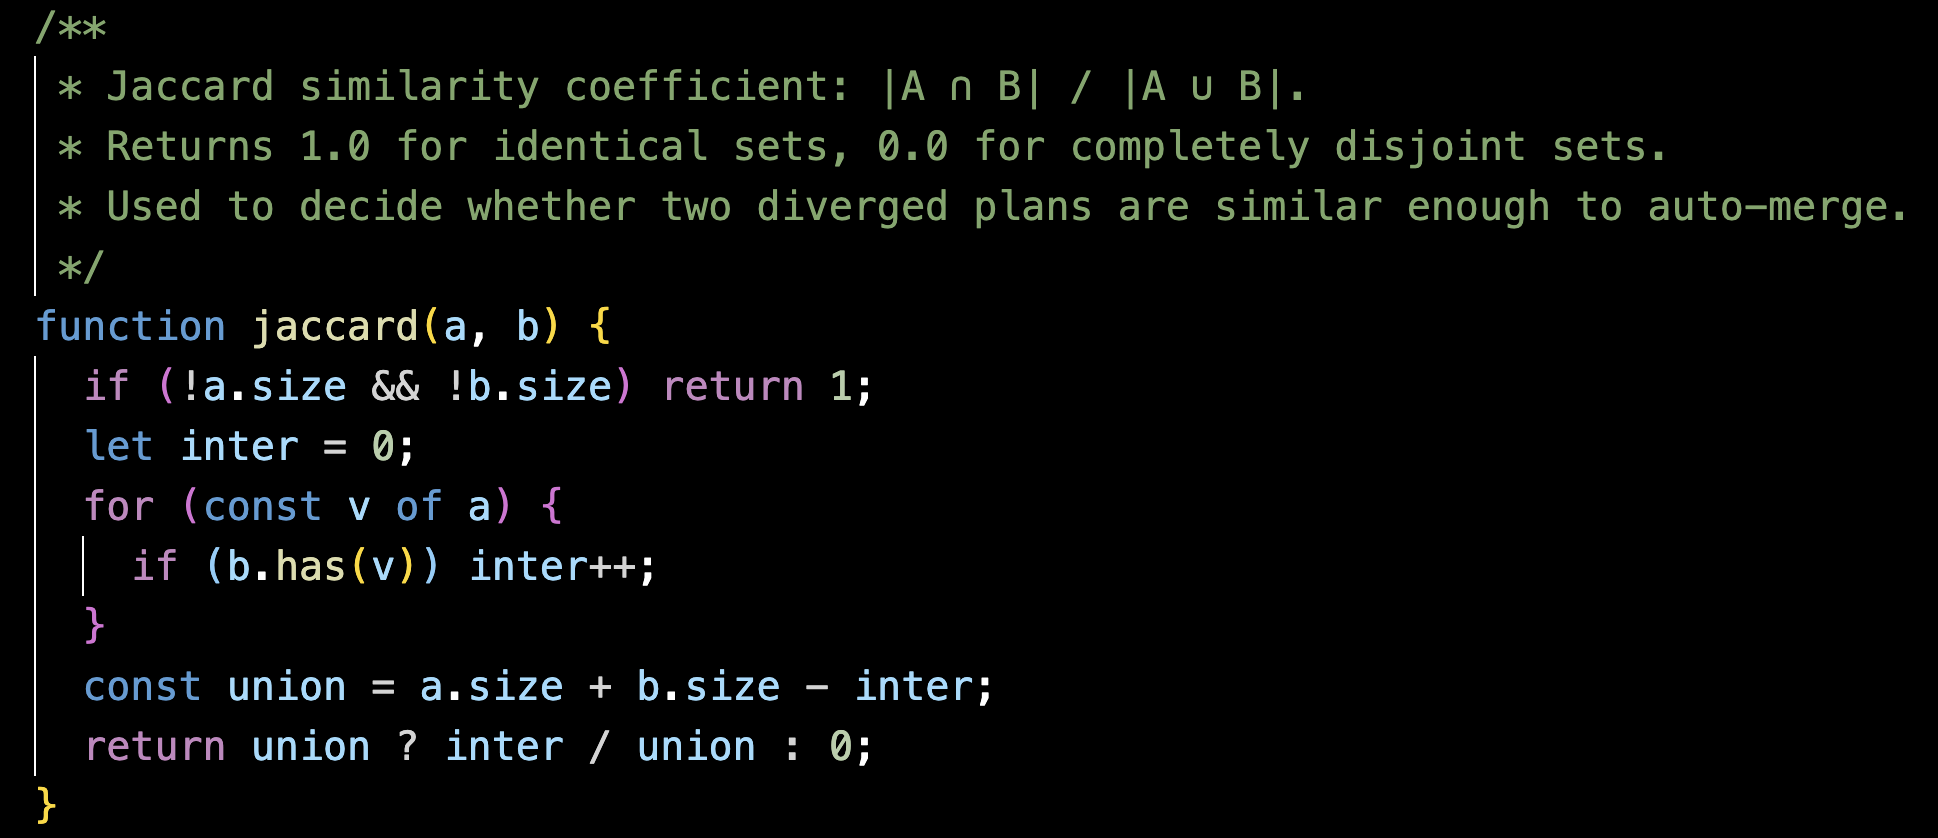
\includegraphics[width=0.85\linewidth]{Chapter6/jaccard-code.png}
  \caption{Jaccard similarity function (\texttt{server/merge.js}).}
  \label{fig:jaccard}
\end{figure}

\section{Routing Implementation}
Routing integration is implemented in \texttt{server/routing.js}:
\begin{itemize}
  \item ORS~\cite{ref_ors_matrix} matrix requests use the matrix endpoint and return durations in
        minutes.
  \item ORS directions requests fetch per-leg geometry for map rendering.
  \item Google Directions~\cite{ref_google_directions_api} transit routes provide detailed per-step segments,
        including polylines decoded via the standard polyline algorithm.
  \item Fallback estimates use Haversine distance with mode-dependent speed assumptions (approximately 5~km/h walking, 15~km/h cycling, 50~km/h driving, and 30~km/h transit).
\end{itemize}

\section{Quick Explore Mode}
Quick explore mode provides a Google-Maps-like workflow where users quickly enter
destinations, optimise an order, and optionally start a repository from the
result. This is implemented via \texttt{server/quickroute.js}:
\begin{itemize}
  \item for small instances (N $\leq$ 12), an exact Held-Karp dynamic programming
        solver is used \cite{ref_tsp_study,ref_tsp_local_search};
  \item for larger instances, NN is used with 2-Opt refinement
        \cite{ref_nn_2opt_hybrid}.
\end{itemize}

The quick route engine builds a travel-time matrix using ORS, transit pairwise
calls for small transit sets (limited to N~$\leq$~7 to control API cost), or
Haversine fallback. Concurrency is bounded to a pool of four simultaneous
requests to reduce API burst risk. The ordering logic reuses the same NN, 2-Opt, and Held-Karp strategies described in Section~\ref{sec:planner-impl} (Algorithms~\ref{alg:nn}--\ref{alg:heldkarp}).

\section{Algorithm Visualisation}
GiTrip includes an educational algorithm visualisation page
(\texttt{server/public/algorithm.js}) that demonstrates three route-ordering
algorithms with step-by-step animation on a Leaflet map:
\begin{enumerate}
  \item \textbf{Nearest Neighbour (NN):} greedy selection of the closest
        unvisited stop; $O(N^2)$ time.
  \item \textbf{NN and 2-Opt:} starts from an NN solution and iteratively reverses
        sub-segments to shorten the route; used for instances with more than 12
        stops.
  \item \textbf{Held-Karp dynamic programming (DP):} exact bitmask DP solver in
        $O(2^N \cdot N^2)$ time; guarantees optimality but is limited to
        N~$\leq$~12 stops due to exponential growth.
\end{enumerate}

The visualisation fetches real routing geometry from the server
(\texttt{/api/algo-matrix} and \texttt{/api/algo-geometry}), supports multiple
transport modes, and includes playback controls (play, pause, step, reset, speed
slider), synchronised pseudocode highlighting, animated scan lines showing which
edges are being evaluated, and a cost comparison panel.

\subsection{Constraint-Aware Scheduling Visualisation}
A second educational page (\texttt{/ui/schedule-demo}) demonstrates the
constraint-aware scheduling algorithm with eight animated scenarios:
\begin{enumerate}
  \item \textbf{Basic Schedule:} cursor-based packing with travel gaps.
  \item \textbf{Opening Hours:} nudging stops forward when proposed before
        opening time.
  \item \textbf{Fixed Time:} immovable stops that other stops pack around.
  \item \textbf{Time Windows:} soft desired-window preferences (e.g.\ lunch
        slot).
  \item \textbf{Day Overflow:} stops spilling to the next day when the active
        window is full.
  \item \textbf{Multi-Constraint:} opening hours, desired window, and fixed
        time combined in a single scenario.
  \item \textbf{Focus Shift:} comparing morning, midday, and afternoon start
        offsets side by side.
  \item \textbf{Compact vs Sparse:} comparing tight and distributed packing
        modes on the same stops.
\end{enumerate}

The page renders a Scalable Vector Graphics (SVG) day timeline (08:00--21:00 for demonstration) with animated stop blocks,
an opening-hours bar, a real-time constraint info panel, and synchronised
pseudocode highlighting. No API calls are required; all data is hardcoded.

\subsection{Three-Way Merge Visualisation}
A third educational page (\texttt{/ui/merge-demo}) demonstrates the three-way
merge algorithm with eight scenarios covering all merge outcomes:
\begin{itemize}
  \item \textbf{Auto-resolved:} clean merge (one side changed), identical
        changes (both made the same edit), and both-delete (both removed the
        same stop).
  \item \textbf{Conflicts:} stop-time conflict, delete-vs-edit conflict,
        field conflict (e.g.\ name differs), file conflict (e.g.\ trip
        description), and whole-plan conflict (Jaccard similarity below~0.4).
\end{itemize}

The page shows four plan panels (Base, Source, Target, Merged Result) with
colour-coded stop cards, animated per-stop comparison, and a file-level
description display for file-conflict scenarios. All three educational pages
share the same visual design, dark colour scheme, playback controls, and
pseudocode highlighting pattern, and are accessible via a ``How it works''
dropdown in the navigation bar.

\section{Frontend Implementation}
GiTrip's pages are server-rendered with EJS templates and enhanced with
client-side JavaScript:
\begin{itemize}
  \item \textbf{Repo UI:} displays trip plan, map, timeline, branches, commits,
        settings, and exports.
  \item \textbf{Merge UI:} presents conflicts and resolution controls, then
        submits a resolution payload to create a merge commit.
  \item \textbf{Planner UI:} collects inputs and submits to the planner endpoint
        to generate a new commit on a planner branch.
\end{itemize}

\subsection{Timeline and Map Editing}
The timeline editor uses draggable SVG elements with snapping to 5-minute
increments. It clamps edits based on travel constraints:
\begin{itemize}
  \item a stop cannot start before the previous stop's departure plus travel
        time,
  \item a stop cannot extend beyond the next stop's arrival,
  \item minimum stop duration is enforced.
\end{itemize}

The map editor uses Leaflet markers with numbered pins \cite{ref_leaflet}. In
edit mode, markers are draggable and route polylines are updated. Transit legs
display additional stop markers and per-leg mode styling (e.g., dashed walking
segments).

\section{Exports and PWA Features}
\subsection{PDF Export}
PDF export is implemented using browser printing (\texttt{window.print()}),
which is robust and avoids server-side rendering complexity.

\subsection{iCalendar Export}
GiTrip generates \texttt{text/calendar} content in iCalendar format and serves
it as an \texttt{.ics} download. The iCalendar format is defined by RFC 5545
\cite{ref_rfc5545}.

\subsection{PWA and Offline}
GiTrip includes PWA support through a web application manifest and a service
worker. The manifest standard is specified by W3C \cite{ref_appmanifest}, and
service workers are defined by W3C as an event-driven background worker model
enabling offline caching \cite{ref_service_workers}. Offline behaviour focuses
on caching core assets and recently accessed pages; limitations include the
inability to guarantee offline routing responses.

\section{Supporting Features}
\subsection{Weather Integration}
Each day in a plan displays a weather forecast retrieved from the Open-Meteo
API. The server fetches daily forecasts (temperature range, precipitation
probability, and weather code) using the first stop's coordinates for each day,
with a 30-minute Time-To-Live (TTL) cache to reduce external requests. Historical data is
fetched for past dates and forecast data for future dates.

\subsection{Travel Alerts}
GiTrip retrieves travel disruption news via the GNews API. City names are
extracted from stop names in the plan, and a search query combining those
cities with disruption keywords (strike, closure, protest, etc.) is issued.
Because articles about upcoming disruptions are typically published before
the affected dates, the search window extends from seven days before the
first trip date through the last trip date, and each article is assigned to the
nearest matching trip date. Results are displayed per day with badge counts.
Users can also add manual alert notes stored in the \texttt{travel\_alerts}
table.

\subsection{Public Gallery with Pagination}
The public gallery (\texttt{/ui/public}) displays trips that owners have
marked as public. The listing supports sorting by recency or star count and
is paginated at 12 trips per page using Structured Query Language (SQL) \texttt{LIMIT}/\texttt{OFFSET}
queries, preventing unbounded response sizes as the number of public trips
grows.

\section{Deployment and Operations}
GiTrip supports deployment via containerisation with a persistent volume for the
SQLite database file (\texttt{gitrip.db}). The server starts on \texttt{PORT}
(default 4000) and automatically increments if the port is in use. Environment
variables provide routing API keys. The system was deployed for Evaluation Day to
allow participants to access the application from multiple machines and personal
devices.
